\chapter{Materials and Methods}\label{chap:methods}
The challenges in genomic analysis of viral material using \ac{NGS} raw read data are a major motivation for this work. Ready-to-use pipelines that can be executed without deeper biological or bioinformatic knowledge specifically designed for the viral genomes of avian influenza virus, poxviruses and foot-and-mouth disease virus are presented below. They run on the Galaxy platform and show that for development of the pipelines, large parts of existing viral genomic analysis pipelines as such for SARS-CoV-2 can be reused and adapted.

\section{Galaxy Platform}\label{sec:galaxy}
Galaxy is a web-based scientific platform that has become a major player in many fields of life sciences and bioinformatics. Founded in 2007, it has provided an emerging amount of resources and tools to empower scientists and researchers to work with biomedical datasets. The platform is free to use and collaborative, as all related codebases are open-sourced on GitHub. Resources on Galaxy cover genomics, metagenomics, transcriptomics, proteomics, drug discovery and non-biology fields like natural language processing and social sciences.\\
Galaxy's primary objective is to make analyses more accessible, reproducible, and easier to communicate among researchers. The platform's distinctive and success is attributed to four core elements: a very active community, public servers, an open-source software ecosystem, and the Galaxy ToolShed. The community adheres to the FAIR practises (Findable, Accessible, Interoperable and Reusable)~\cite{10.1093/nar/gkac247}.

The Galaxy community is thriving, with over 124,000 users who also contribute to subcommunities. The servers for analyses provide access to public datasets and workflows. The open-source software ecosystem ensures automated setup and deployment of all tools and services, making it simple for beginners and professionals to use. The Galaxy ToolShed is a server dedicated to hosting, sharing, and installing tools used on the platform. A Galaxy tool is the abstraction layer that makes external software usable from within Galaxy with a front-end, and lets users start the program with all its parameters and inputs from within Galaxy. Each program that is available as a Galaxy tool is XML-wrapped to make dependency requirements, parameter and data inputs and other settings possible via the Galaxy web-interface. \\ 
Galaxy workflows are a key feature that allow the user to stack tools in a chain and to configure them so that the workflow user only has to upload or enter data for the input fields. The automated subsequent order and execution of tools in a workflow is used for modular, longer analyses that are executed repeatedly. Each user can register for free and has a default of 250 GB disk space allocated on the three main public Galaxy servers to run computations. \\
Workflows that are available on and accepted by the \ac{IWC} on GitHub are conforming with the community's best practise standards and tested on the latest Galaxy release. Dockstore for availability in the U.S. and WorkflowHub for EU users publish the \ac{IWC} workflows and guarantee the availability in Docker-based environments and on the workflow collaborative WorkflowHub~\cite{o2017dockstore, goble2021implementing}.

Important contributions of Galaxy, as stated by the Galaxy Community (2022), include Vertebrate Genome Project assembly workflows and research collaborations about \ac{SARS-CoV-2}. Another toolkit leveraged in Galaxy is Galaxy-ML, a set of tools that form a suite for analyses based on machine learning. With growing publicity, more topics are covered by and moved to Galaxy. It has contributed to over 5,700 scientific publications and has many tutorials available for researchers to use. \\
The Galaxy platform is continuously enhanced, and it still attracts around 2,000 new users every month, indicating its quality and significance. The team and infrastructure of Galaxy initially come from the Nekrutenko lab in the Center for Comparative Genomics and Bioinformatics at Penn State, the Taylor lab at Johns Hopkins University, and the Goecks Lab at Oregon Health \& Science University. There are 138 public servers available worldwide as of 2023, while the three most prominent general-purpose server instances are hosted by teams at University of Freiburg, Germany, for \href{https://usegalaxy.eu/}{UseGalaxy.eu}, Texas Advanced Computing Center for \href{https://usegalaxy.org/}{UseGalaxy.org} and Genomics Virtual Laboratory, formerly at the University of Queensland, for \href{https://usegalaxy.org.au/}{UseGalaxy.org.au}. These three public servers are synchronised in a subset of reference tools~\cite{10.1093/nar/gkac247}. \\
The platform serves as a public infrastructure that can be used in many contexts and by professionals from all fields and backgrounds. It therefore is very suitable for offering publicly available and transparent resources for disease surveillance.

\section{SARS-CoV-2 Workflow}
The \ac{COVID-19} pandemic motivated many researchers to study and develop analysis workflows of \ac{SARS-CoV-2} sequencing data. In the \ac{IWC} repository, there are seven workflows available and ready to use on Galaxy for the different kind of \ac{NGS} data (ONT/Illumina) and with varying objectives (variant calling/variation reporting/consensus construction). Specifically for Illumina ARTIC reads, a workflow for genomic analysis based on the \texttt{iVar} suite has been released~\cite{iwc2021covidivar}. It is conceptually similar to other existing pipelines outside of Galaxy, written in Nextflow, Snakemake and \ac{WDL}. The workflow for ampliconic Illumina paired-end reads consists of the following steps: (1) read adapters are trimmed with \texttt{fastp} and (2) mapped to a reference genome with \texttt{BWA-MEM}. The user is required to select an appropriate reference for mapping of the reads. The alignment is (3) quality filtered using \texttt{Samtools view}, keeping the reads with a minimum length of 20 and only if they are mapped and properly paired. After generation of quality and coverage reports, (4) \texttt{iVar trim} is run with the primer scheme to cut out the primers from the filtered alignment. The cleaned alignment file is processed (5) with \texttt{iVar consensus} to call the consensus sequence and (6) with \texttt{iVar variants} to call variants. The resulting output files are used for variant annotation, phylogenetic assignment of the outbreak lineages and clade assignment. The workflow skeleton is depicted in~\figref{fig:3-sars-wf}. 

\begin{figure}[h!]
	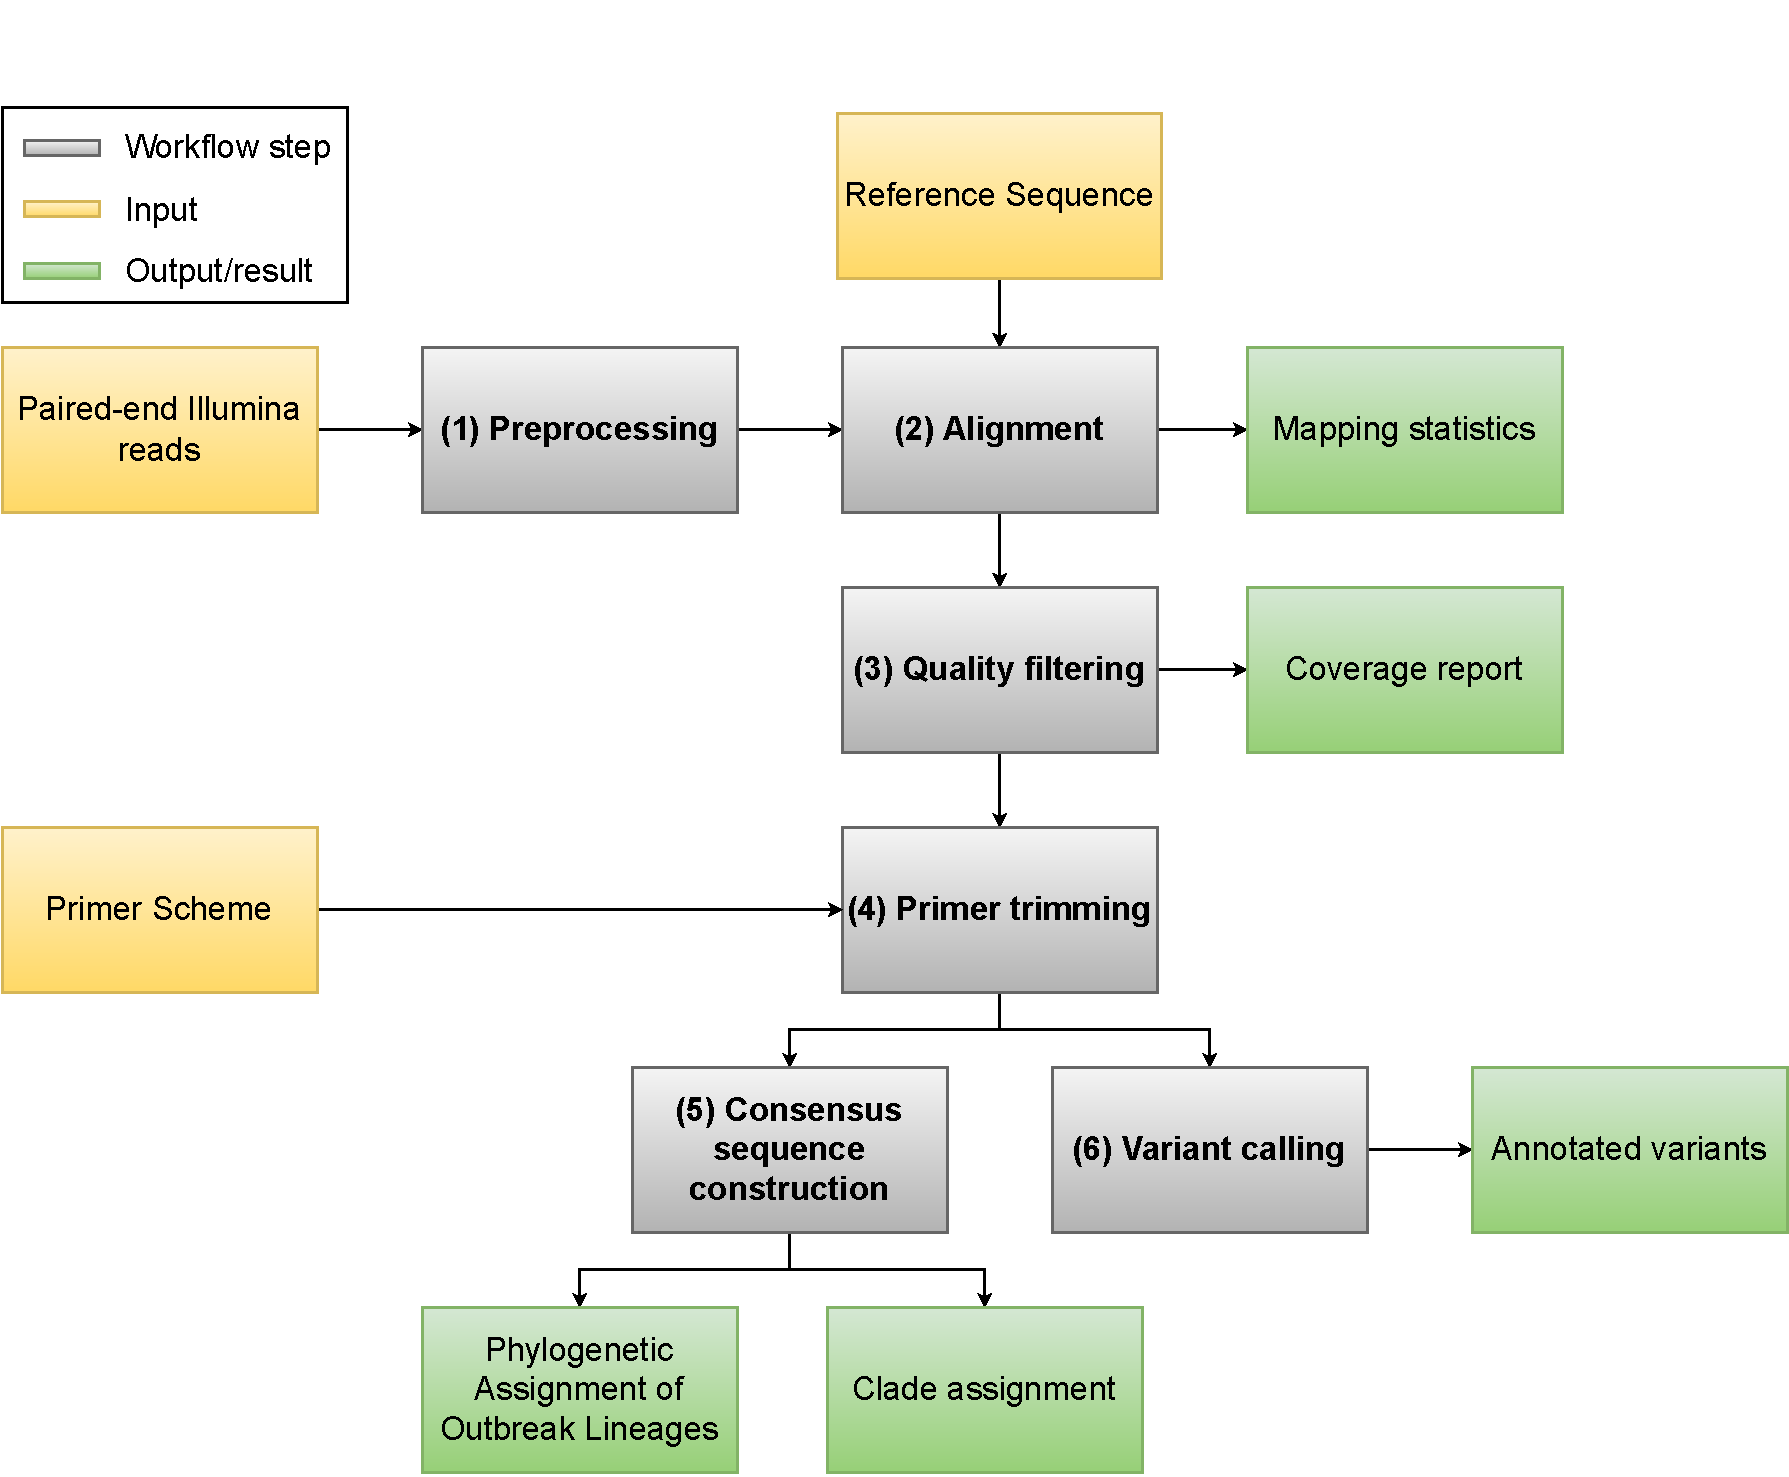
\includegraphics[width=0.95\textwidth]{media/3-sars-cov-2.pdf}
	\caption{Simplified SARS-CoV-2 analysis workflow for ampliconic Illumina-sequenced data.}
	\label{fig:3-sars-wf}
\end{figure}

This workflow is designed for the specific attributes of the \ac{SARS-CoV-2} genome and addresses the complex task of consensus construction by aligning reads to a reference, however other viral genomes can be analysed on genomic level in similar ways. Accounting for the genomic structure and composition of each virus, analysis workflows for poxviruses, avian influenza virus and foot-and-mouth disease virus are developed in this work, reusing components of the described \ac{SARS-CoV-2} workflow. The requirements for the viruses and the workflows are described below, before the developed workflows are examined.

\section{Workflow Requirements}
To account for the distinct attributes of the viruses, automated pipelines used to achieve whole-genome insights from raw reads must be tailored accordingly and aspects like speed, accuracy and reliability of the tools are considered. The requirements for each workflow are explained below.

\subsubsection{Requirements for Poxvirus Analysis Workflow}
As explained in~\secref{sec:2-pox}, the genome of poxviruses is bound by identical sequences located at both termini of the genome. It is shown that the size of such differs for some poxviruses like rabbitpox and vaccinia virus, Capripoxviruses have shorter \acp{ITR} with circa 2.2 to 2.4 kilobases~\cite{wittek1978inverted}. For a whole-genome reconstruction from \ac{HTS}-generated reads, alignment algorithms look for the unambiguous location of a read to find the most agreed position for a complete alignment. Since there is no unambiguous position for repeated identical sequences neither in reference-based mapping approaches nor \textit{de novo} assembly, a new approach has to be used so that the two \acp{ITR} are not aligned in the same run, but separately to constitute disambiguity. Therefore, a method that splits the sequencing reads into two parts, separating the identical sequences and running alignment algorithms for each of the splits was developed. To build the full-length consensus genome, the alignments need to be ``glued'' back together. To ensure the reads to be mapped in the appropriate and not in the incorrect \ac{ITR}, the reads need to be sequenced in two pools with overlapping amplicons. A similar tiling amplicon protocol has been described by Mathijs et al. and the ARTIC network for \ac{SARS-CoV-2} data~\cite{tyson2020improvements, mathijs2022robust}. \\
As a consequence, a requirement for a reference-based surveillance of the genomics of poxviruses is the availability of the primer scheme that was used for the split amplicon-based sequencing with an Illumina sequencer. Working with Illumina-generated \ac{NGS} data, the workflow necessitates a quality control and trimming of the reads to remove sequencing artefacts and adapters. The \ac{BED} file containing the primers, their positions and the pool identifiers is essential for the correct linking of the alignments when splitting the pipeline into two parts and merging them back together. Mapping of each genome-half that each contains one \ac{ITR} requires a reference sequence, which is a compulsory and essential workflow input. Since reads from both genome halves are mapped to the same reference, although different parts, the reference genome needs preparation, so that reads are unambiguously mapped. Therefore, a masking of the reference helps to allow the mapping to only one half of the genome. As the sequencing in two pools cannot obtain reads in perfect halves due to amplicon and primer designs, the boundaries of masking the reference can be computed by the positions of the primer sets that split the pools. \\
Apart from the split approach with a masked reference sequence for alignment, the poxvirus reads can be processed similarly as \ac{SARS-CoV-2} reads. In the \ac{SARS-CoV-2} workflow, clade and lineage assignment, with \texttt{Nextclade} and \texttt{Pangolin} respectively, work with \ac{SARS-CoV-2} specific databases. Although the tools are designed to work with the \ac{SARS-CoV-2} genome, the \texttt{Nextclade} tool is adapted and expanded to work with other viruses (mpox, Influenza A H1N1 and H3N2 HA gene, Influenza B Victoria and Yamagata HA), however currently not suitable for undetermined poxvirus genus members~\cite{aksamentov2021nextclade}.

\subsubsection{Requirements for AIV Analysis Workflow}
The main objectives for surveillance of \ac{AIV} on the genetic level are to get phylogenetic insights and to check for mutations or new variants that occur in the \ac{HA} and \ac{NA} proteins as a consequence of reassortment events. \\
A pipeline for an avian influenza virus sample that builds a consensus sequence from raw reads requires a reference sequence that it can align the \ac{NGS} reads to. For an Illumina-based workflow, preprocessing is crucial to ensure reliable results working with the reads. Quality filtering and trimming must be included in the beginning of the workflow. A main caveat of many existing pipelines for \ac{AIV} genomic analysis is the user's choice of reference sequence, since it is an arbitrary selection and has a direct impact on the alignment. Since the reference should be as similar as possible to the aligned genome reads in order to detect point mutations and detect minor assets, this is a key factor for the quality of the consensus sequence. Another, computationally more expensive approach for alignment is an assembly, which does not require a reference sequence. Since the influenza segments can have very similar regions at the segment's ends and mapping generally is computationally faster than assembly, a reference-guided mapping method is favoured for the analysis of \ac{AIV} samples due to the genome size and high mutation rates of \ac{AIV}. The goal is to use a reference that is representative of the sample being analysed. In the \ac{SARS-CoV-2} pipeline, it is recommended to use a reference genome from a recent \ac{SARS-CoV-2} strain. For avian influenza virus, multiple reference sequences exist depending on the strain and subtype, however this information only helps for the reference selection if the strain or subtype of the sequenced sample is known. Additionally, avian influenza viruses tend to reassort during replication and one sample may match with different possible references for the different segments. Taking a single reference for mapping, a possibly new reassortment event may not be discovered. Hence, a dynamic approach that is sensitive enough for the segmented structure of the \ac{AIV} genome is needed to pick a representative reference. A search tool like \texttt{VAPOR} could help identify close reference sequences based on the input reads by looking up a large user-defined database of sequences. The diversity of \ac{HA} and \ac{NA} segments' sequences is significant enough to make it challenging to map sequenced reads to a single, full-length influenza A reference sequence. Although an approach that takes any (maybe imperfect) reference strain may be effective for the other six segments, the mapping software would frequently be unable to achieve sufficiently plausible matches for sequenced reads of the \ac{HA} and \ac{NA} segments. By introducing a method that finds the best reference sequence from a database, the expensive \textit{de novo} assembly is avoided, the user is not required to choose an arbitrary reference and mapping to a suitable reference with minimal bias can finally be performed. \\
Compared to analyses with genomes such as \ac{SARS-CoV-2} and due to the segmented structure of the \ac{AIV} genome, duplicates among the mapped reads of the \ac{AIV} sample should not be dismissed as they are in the \ac{SARS-CoV-2} workflow, but kept for maintaining a reasonably high coverage for the further analysis. Downstream analyses for phylogenetic placing are useful for the \ac{HA} and \ac{NA} genes to trace viral origins and consider relations to similar strains, as well as visual summaries of \acp{SNP} for identification of genetic variation in different regions.

\subsubsection{Requirements for FMDV Analysis Workflow}
Genomic analysis of the viral \ac{FMDV} \ac{RNA} genome requires a workflow that accounts for its high mutation rate and takes into account the short genome length. Aligning raw Illumina-sequenced reads requires quality control in a preprocessing step to remove sequencing platform specific adapters and dismiss reads with low quality. For alignment of the reads to construct a consensus sequence, mapping to a reference or assembly of the reads are considered. Finding a representative reference from a database with many sequences, for \ac{FMDV} reads this approach would regularly fail due to the very high mutation rate and ensuing large differences between the query reads and the database sequences. Therefore, a different approach to find a suitable reference sequence for mapping is required. Since the \ac{FMDV} genome is relatively short with approximately 8.3 kilobases, a \textit{de novo} assembly takes only little amount of computational resources for a run. This is due to less contigs to assemble and fewer gaps to fill during assembly, and usually more high coverage regions that facilitate the assembler to find long contigs. The overall complexity of \textit{de novo} assembly is highly reduced with short genome lengths and therefore increases efficiency of assembly.\\
A \textit{de novo} assembly of the \ac{FMDV} reads to avoid an arbitrarily chosen reference sequence with a subsequent \ac{BLAST} search in the nucleotides database is one method to find similar sequences that allow for a high-quality mapping and consensus sequence construction.\\
Additionally, taking up concepts from the \ac{SARS-CoV-2} workflow, the pipeline should include steps for quality control, including the removal of low-quality reads and the identification and removal of potential contaminants or other sources of error. Finally, a workflow for \ac{FMDV} genomic analysis should accommodate Illumina-sequenced data and be able to scale up for working with multiple samples at a time.

\section{Workflow Development}
The developed Galaxy workflows for poxviruses, \ac{AIV} and \ac{FMDV} that account for the genomic structure of each virus and the \ac{NGS} approaches are described below.

\subsection{Poxvirus Illumina Workflow}\label{sec:pox-wf}
The newly designed Galaxy workflow for Illumina-sequenced poxvirus samples with a tiling amplicon approach is available on WorkflowHub, Dockstore and on \ac{IWC} to use on the Galaxy EU server. Links can be found in Supplementary~\secref{sec:apx-pox-links}. \\
This workflow is the first public pipeline for Illumina-sequenced data that provides a ready-to-use infrastructure for genomic analysis of poxviruses with ampliconic data that were sequenced in two pools and combines a wet lab approach with bioinformatic tool sets. It aims at constructing the consensus genome from ampliconic Illumina-sequenced reads by reference-guided mapping and providing alignment files, sample-specific consensus sequences and intermediate results and reports that give insights into reads, mapping quality and mapping coverage. The pipeline is clearly shown in its structural elements in~\figref{fig:3-pox-wf}. \\ 

\begin{figure}[ht!]
	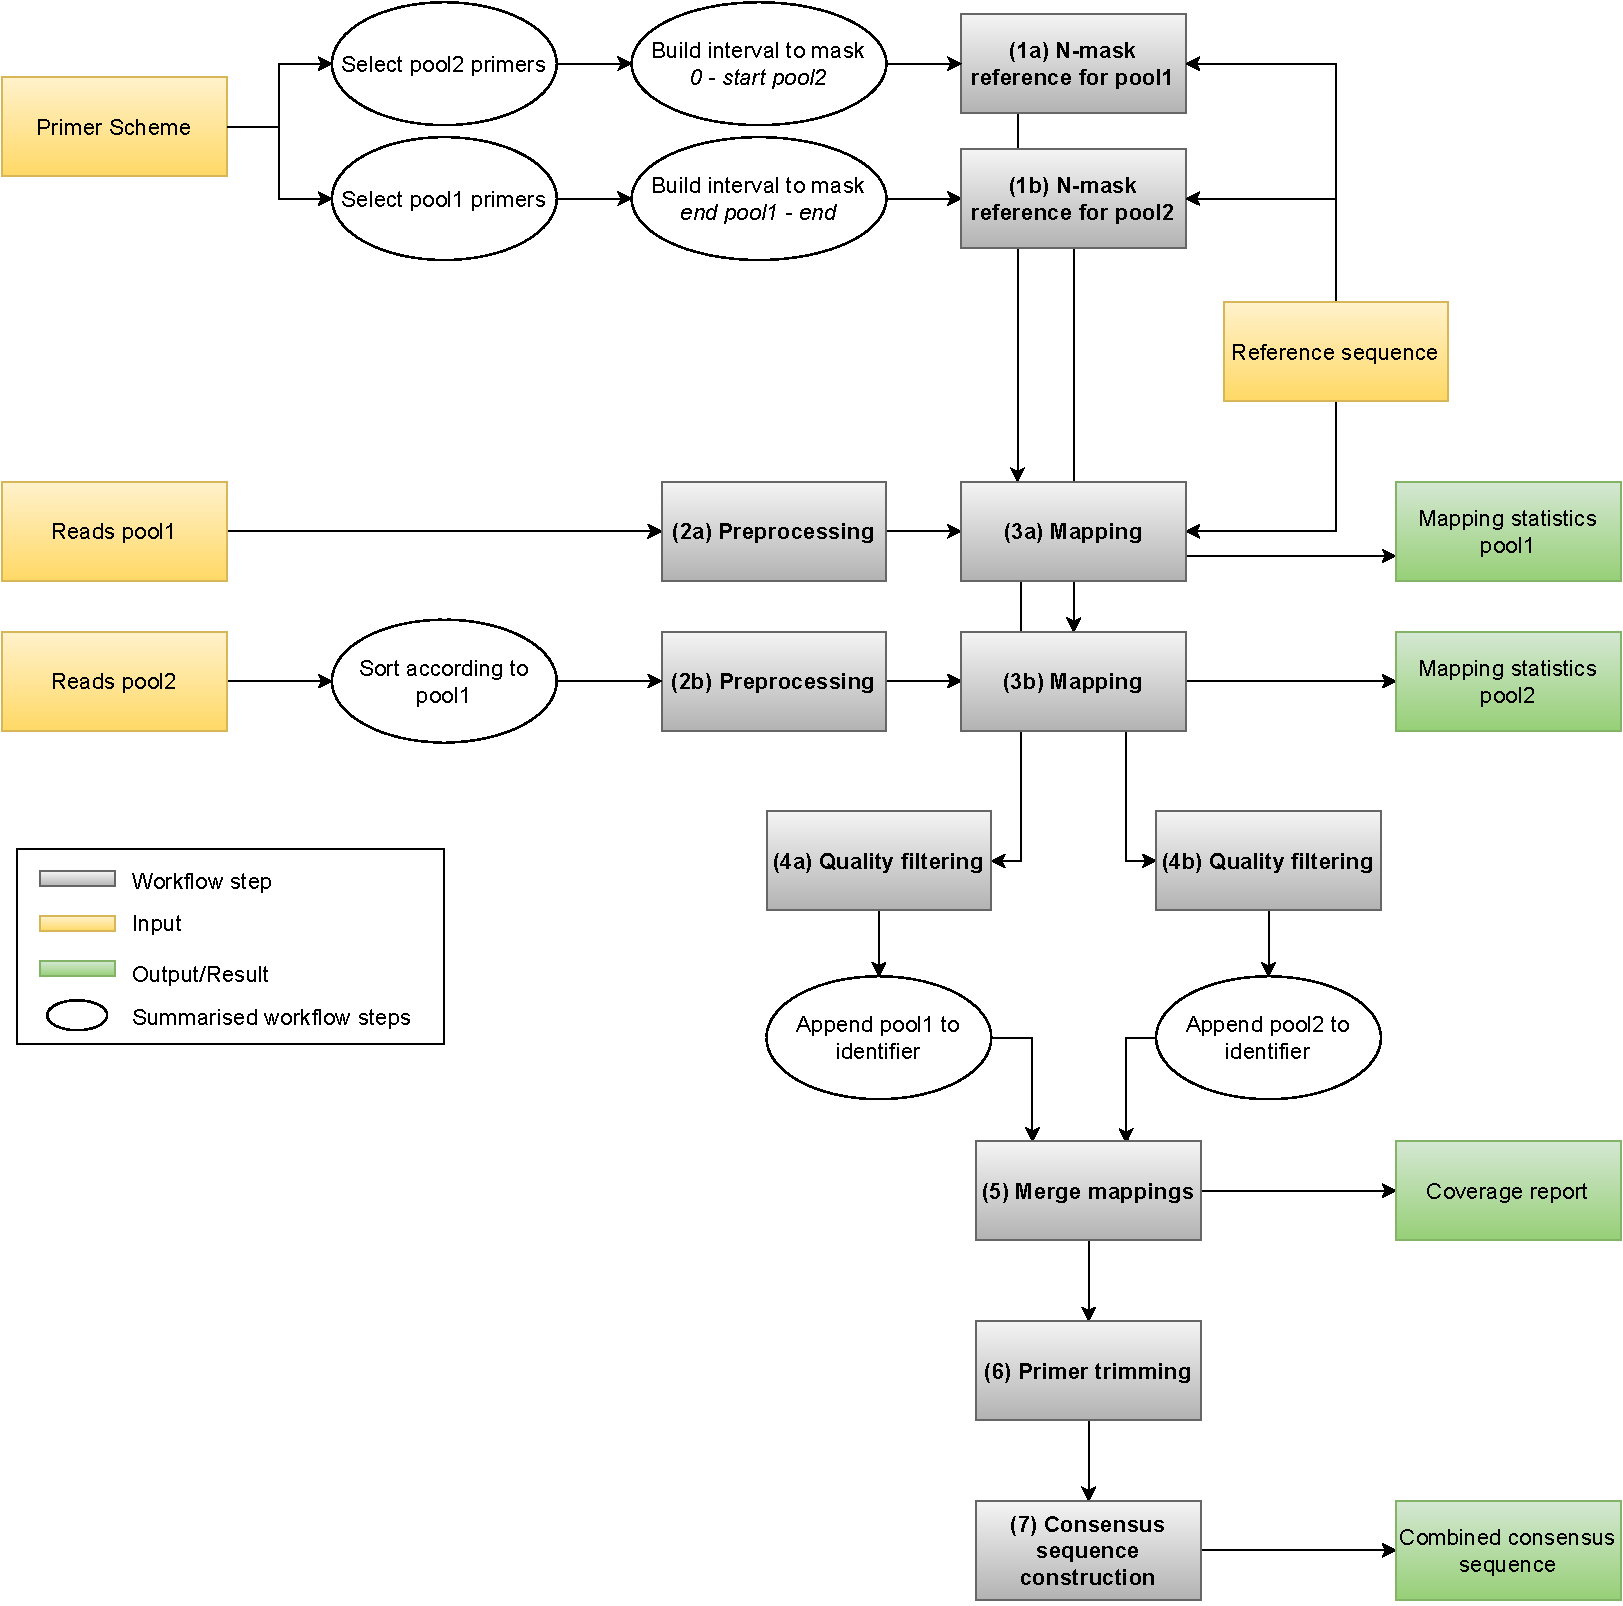
\includegraphics[width=0.92\textwidth]{media/3-pox.pdf}
	\caption{Simplified poxvirus genomic analysis workflow for ampliconic Illumina-sequenced data.}
	\label{fig:3-pox-wf}
\end{figure}

To account for the repeated \acp{ITR} at the ends of the poxvirus genome, the workflow is based on a tiled amplicon approach that separates the \acp{ITR} during reads alignment to ensure unambiguous mapping of reads. Therefore, the workflow requires the input reads in two sequencing pools that each represent one half of the genome and, importantly, include one of the repeated \acp{ITR} each. During the first steps of the workflow, the reads of the two pools are processed individually as half genomes. Input data for the workflow are two distinct collections of reads from \textit{pool1} and \textit{pool2}, sourced from the sequencing in Illumina paired-end mode and separately sequenced for the 5' and 3' half; the used primer scheme in \ac{BED} file format that contains an indicator for \textit{pool1} or \textit{pool2} in the \textit{SCORE} (5th) column; and a reference sequence that is used for mapping which can be retrieved from the \ac{NCBI} reference sequence database depending on the genus of the sequenced sample. \\

\begin{figure}[ht!]
    \centering
    \hspace*{-8pt}
    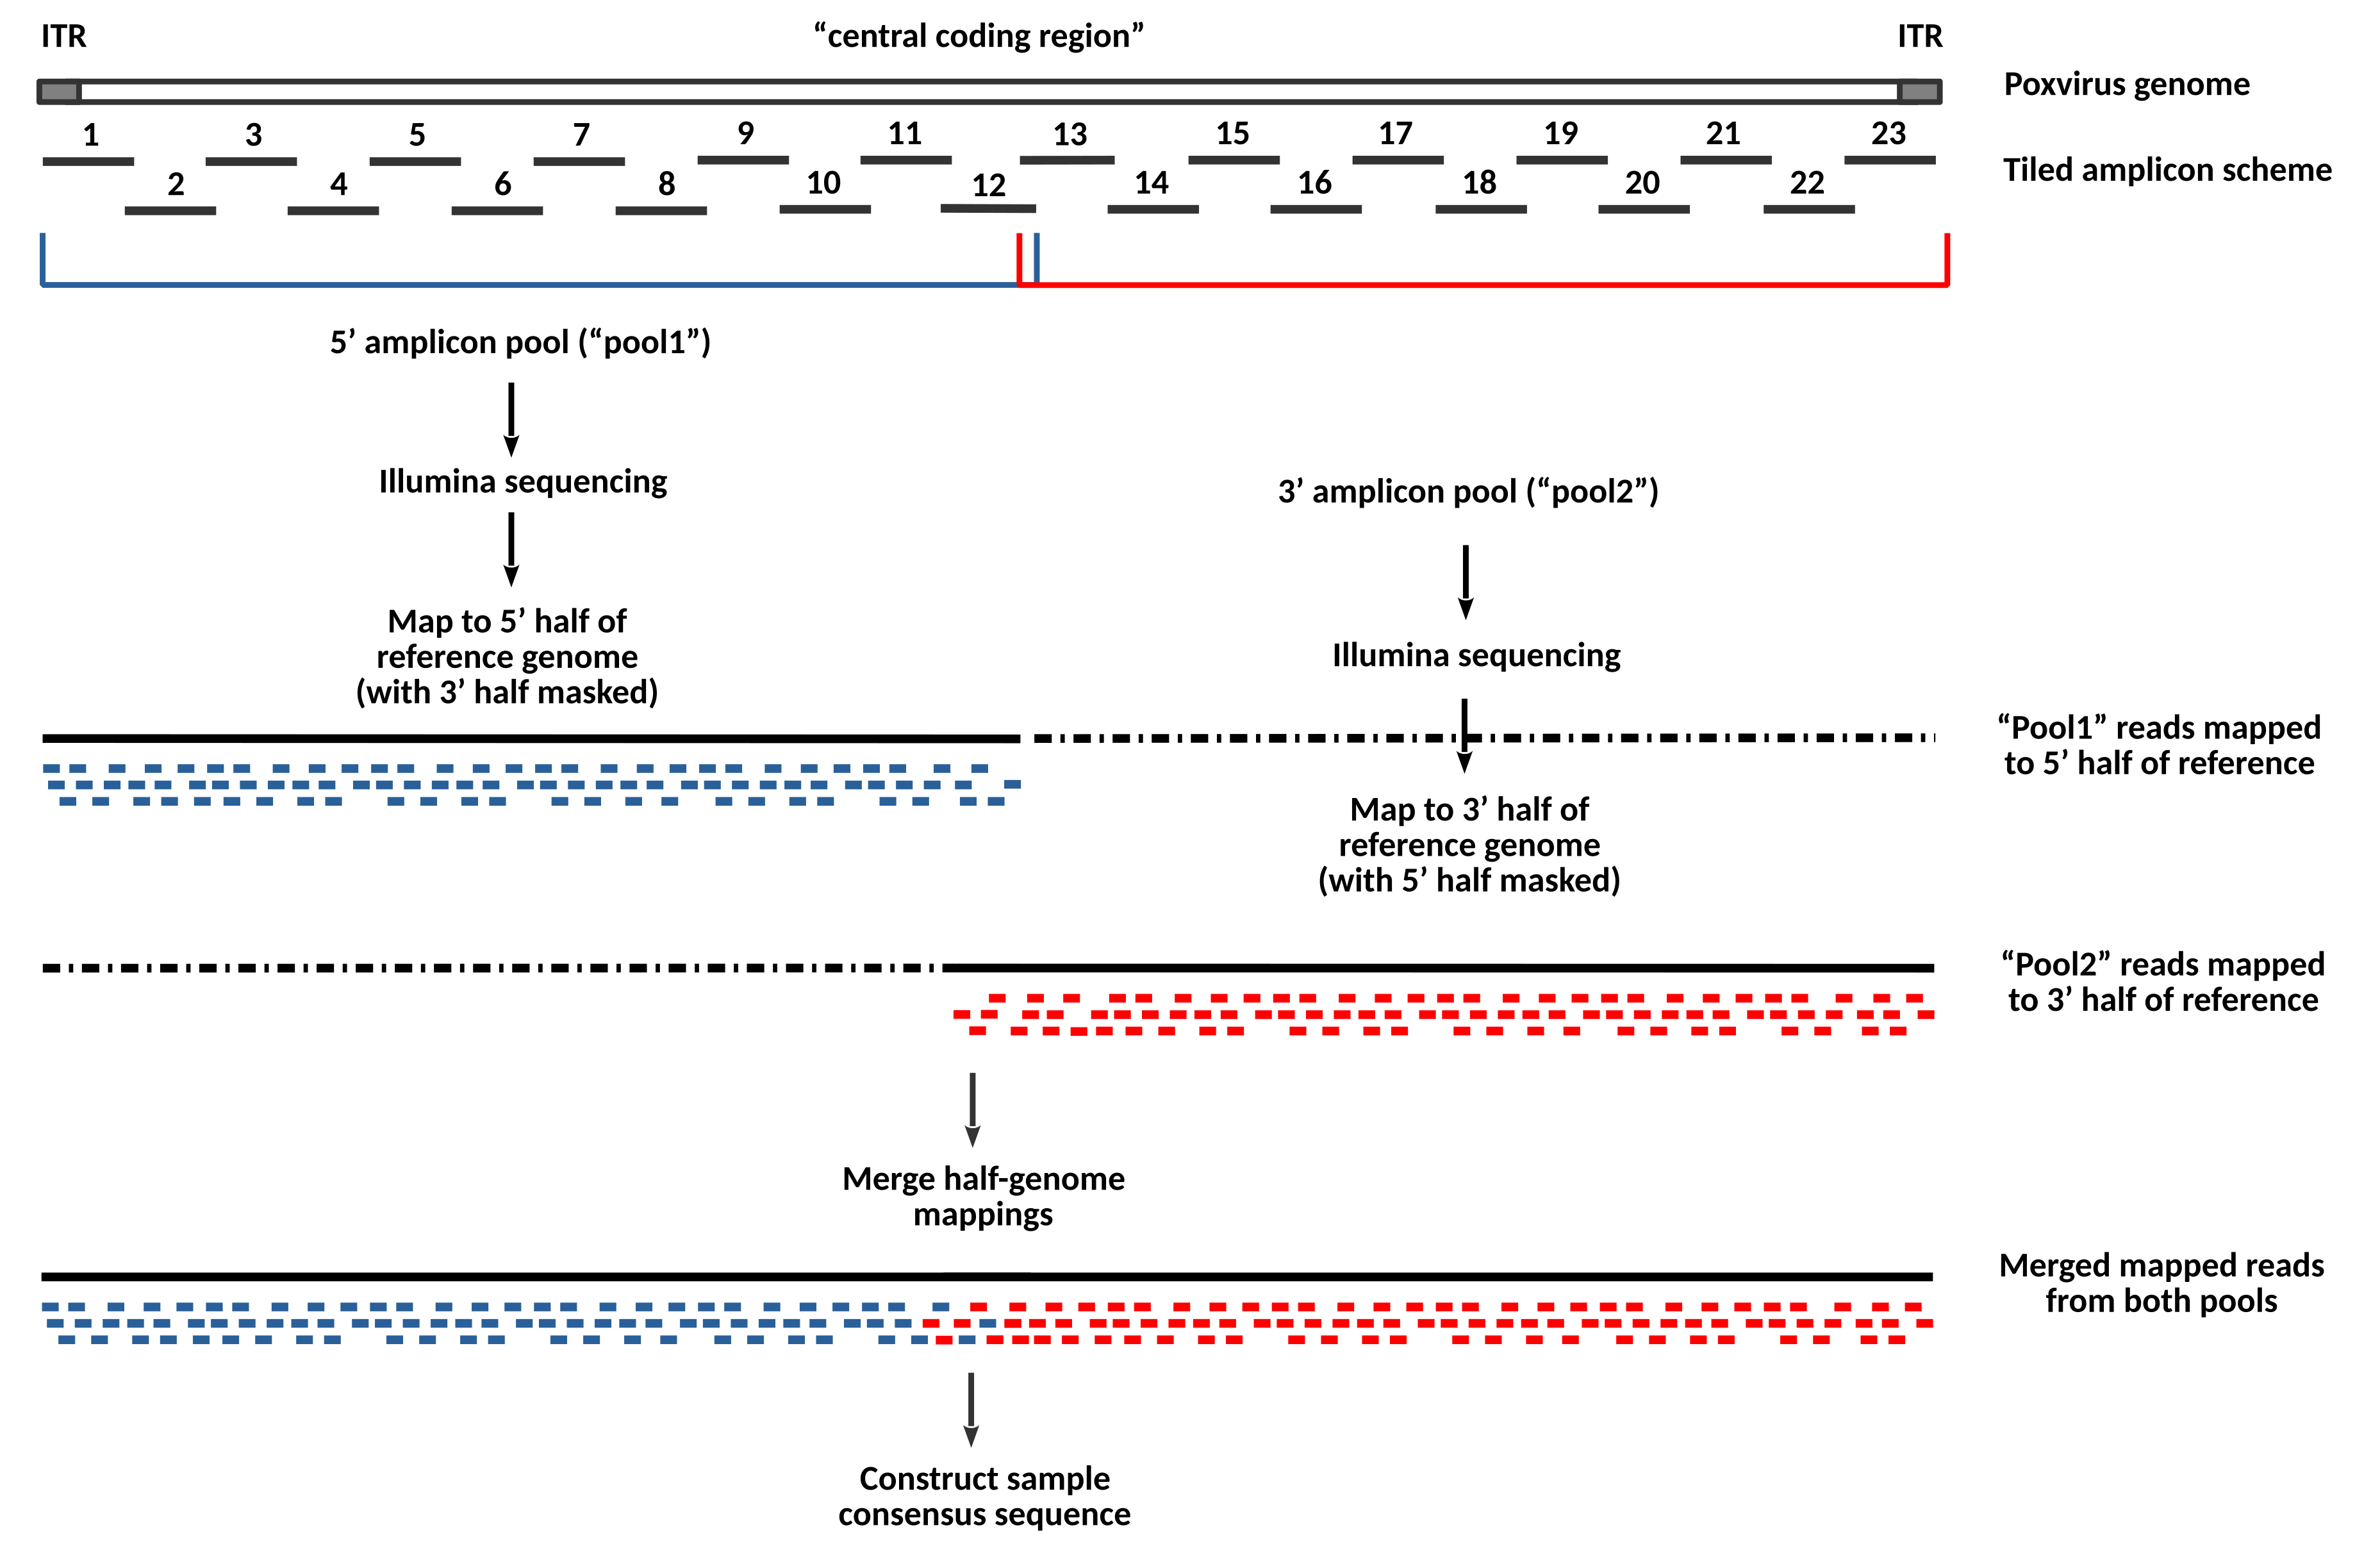
\includegraphics[width=1.1\textwidth]{media/4-pox-ampl-fig.png}
    \caption[Tiling amplicon scheme used in poxvirus workflow.]{Tiling amplicon scheme for wet lab amplification, emphasising masking of the reference, mapping in two pools with two multiplex PCR reactions each and merging of mappings with almost no overlap. Source: adapted from Galaxy training material supplementing this workflow, available via link in Supplementary~\secref{sec:apx-pox-links}.}
    \label{fig:3-pox-ampl}
\end{figure}

As a first step, (1) the provided reference sequence is prepared for the mapping of the two read pools. Hence, the primer scheme is needed to determine the start and end position of the two pools so that the remaining bases can be N-masked. For mapping \textit{pool1}, which accounts for the 5' half of primers to the full-length reference, the 3' half of the reference sequence is N-masked and therefore the boundaries for the remaining bases are introduced as a text parameter for further workflow logic. The N-masking of the reference starts at the minimal start position of the first primer of \textit{pool2}. If the pools and amount of primers are of similar size, this position is in the middle region of the reference sequence. It is important that this position, separating the pools, is in between the two \acp{ITR}, so the individual mappings of each pool only contain one \ac{ITR} each. Accordingly, for the mapping of \textit{pool2}, the interval of the remaining bases is determined by taking the maximal end position of the \textit{pool1} primers and the full length of the reference sequence as an end position so that the masking of the first half can be conducted. The construction of the text parameters in the correct input format is done by multiple Galaxy-specific text-processing tools. This concept, including even and odd numbered amplicons for each pool, is visually illustrated in~\figref{fig:3-pox-ampl}, with the 5' genome half depicted in blue and the 3' genome half in red. \\
Using this approach, it is ensured that the \acp{ITR} are unambiguously mapped, and coverage statistics are expressive, which would not be the case if mapping would be performed on the unmasked full-length reference and reads from the \ac{ITR} regions could be mapped to either \ac{ITR}.\\
The poxvirus workflow is designed to process multiple samples in one run. The workflow requires the raw reads to be uploaded in two distinct collections with the forward and reverse reads each, one for \textit{pool1} and one for \textit{pool2}, each containing the reads for potentially multiple samples. For better comparison during the workflow, the samples in the second reads pool collection are sorted in the order of how they are listed in \textit{pool1}. This reordering is part of the workflow before other steps are induced.\\
Before mapping, (2) the reads of both pools are preprocessed with default settings of \texttt{fastp} to automatically trim Illumina-specific polyG tails of the reads and remove sequencing adapters with default settings of \texttt{fastp} to ensure quality filtering and remove reads with very low quality and short length. \texttt{fastp} defaults to lenient parameters that allow most of the Illumina-sequenced reads to pass. The quality threshold is adjusted to a minimum of Q30, which is still a relaxed value considering working with Illumina-sequenced data that usually come in high quality.\\
The following (3) mapping step with \texttt{BWA-MEM} takes the corresponding masked reference sequence for each genome-half as explained. A statistics report for each alignment is generated using \texttt{Samtools stats} and allows the user to inspect the mapping quality and coverage of the alignments on the reference. Next, the alignments are (4) filtered for quality using \texttt{Samtools view} to keep reads with a minimum length of 20 and only properly paired and mapped reads. These steps are conducted separately for each read pool. Additionally, the read group identifiers (\textit{pool1/pool2}) are prepended to the \ac{BAM} header so that when using external software, the pool and sample identification is assured and unambiguous for the user. In the next step, (5) the two alignments are merged while still retaining the identifiers for each sample and pool. This step requires the alignment datasets in a specific format to not merge all sample's alignments to one. Therefore, the Galaxy specific tools \texttt{Apply rules} and \texttt{Zip Collections} are applied to create the nested collection in its required format. For the full-length mapping, a coverage report is generated with \texttt{QualiMap BamQC} which allows the inspection of the alignment quality and to examine the part where the mappings are merged together. The mean coverage depth is an important standard parameter when performing \ac{NGS}. It indicates how often each base occurs on average in the individual reads. For smaller segments or amplicon-based data, checking the depth of coverage on the entire reference length is crucial as it provides information on how close the sequenced sample is compared to the reference sequence that was selected for mapping. Low coverage of an alignment indicates incorrect mapping due to genetic differences or low read quality. Therefore, coverage plots are provided in the workflow for each sample.\\
To prepare the merged alignment for consensus sequence construction, (6) primer-trimming with \texttt{iVar trim} masks the primer ends. Like this, it is ensured that the primers are not weighted during consensus construction. The (7) consensus sequence is called with \texttt{iVar consensus} and a 50-fold minimum depth. For this step, the user can either use provided workflow-defined default settings (minimum quality score to count base: 20, minimum allele frequency threshold to call \ac{SNV}: 0.7, minimum allele frequency to call indel: 0.8) or enter their own values before starting the workflow. These settings yield for the minimum of 50 sequenced reads per base in coverage, and require at least 70\% of the reads at one position to suggest the same base in order to call consensus, and a minimum of 80\% agreement for indels. With the final combined consensus sequence in FASTA format, combined to a single multifasta file for each input sample, further downstream analyses can be started after the workflow has finished.

\subsection{AIV Illumina Workflow}\label{sec:aiv-wf}
We designed a fully automated pipeline for the analysis with a reference-based mapping approach of Illumina-sequenced reads in paired-end mode from avian influenza samples. The workflow is integrated in the Galaxy platform and is available with all related material via links provided in Supplementary~\secref{sec:apx-aiv-links}. Furthermore, to the best of our knowledge this pipeline is the first ready-to-use workflow that uses a hybrid reference sequence for a fast mapping and provides various outputs for downstream analyses. It is designed to take one input sample at a time and quality reports are emitted during the workflow run. The outputs of the individual analysis steps can be used for any consecutive research based on the user's objectives. The \ac{AIV} workflow is outlined in~\figref{fig:3-aiv-wf}, where the nine main steps of the workflow are visualised. A link to the full workflow and its supplementary material can be found in Supplementary~\secref{sec:apx-aiv-links}.\\
One novelty of our \ac{AIV} workflow is the consideration of the different segments of the influenza virus genome in the composition of the reference sequence. After uploading paired-end Illumina-reads and a reference database, the workflow builds a hybrid reference from the database for each of the genome segments. The reference sequence database is described in detail in the subsequent~\secref{sec:3-aiv-ref}. If a user decides to upload their own curated references, it is important to follow the sequence identifier pattern so that the extraction of sequence identifiers during the workflow works as expected: \\ >\textit{segment\_name$\mid$influenza\_strain$\mid$subtype$\mid$accession\_number}\\ Spaces must be avoided and can be replaced by underscores. For instance, this is one entry's identifier (followed by the nucleotide sequence in the next line): \\ >\textit{PB1$\mid$A/duck/Manitoba/1953$\mid$A/H10N7$\mid$KF435047.1} 

\begin{figure}[ht!]
	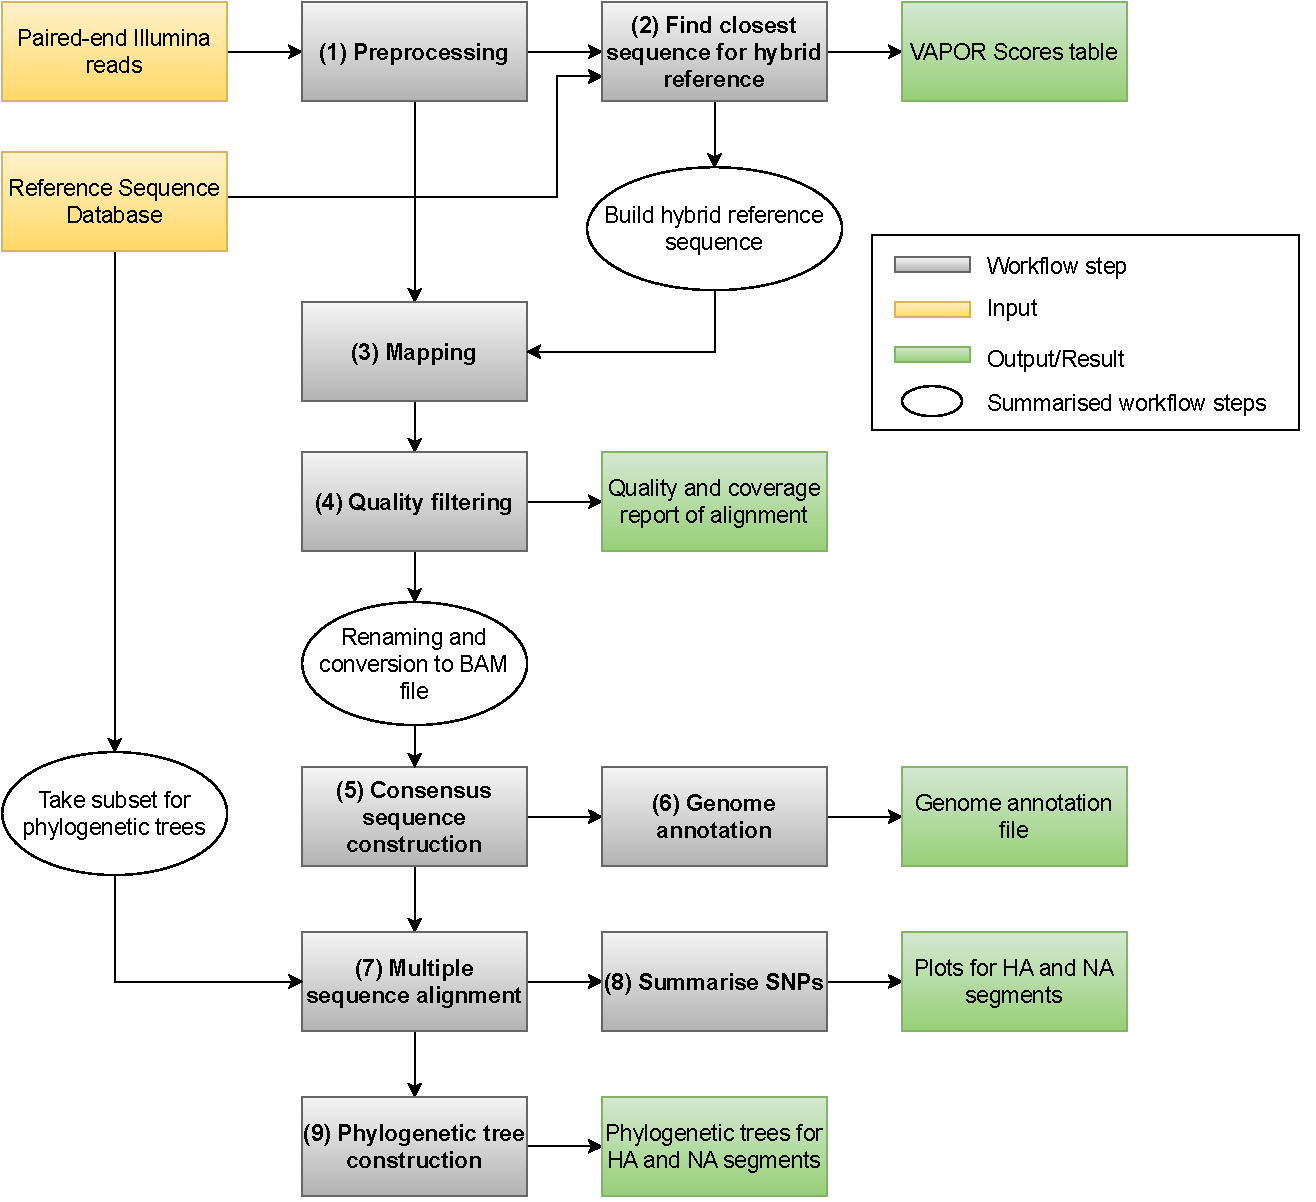
\includegraphics[width=0.88\textwidth]{media/3-aiv.pdf}
	\caption{Simplified \ac{AIV} genomic analysis workflow for Illumina-sequenced data.}
	\label{fig:3-aiv-wf}
\end{figure}

The \ac{AIV} workflow takes the reference sequences in single input datasets split by segment and the Illumina-sequenced forward and reverse reads, and an additional numeric parameter to determine the size of the produced phylogenetic tree. After (1) preprocessing of the reads with \texttt{fastp} with default quality trimming options, and additionally to dismiss reads shorter than 30 bp, filter out 5' and 3' ends with a mean quality of below Q30 (a Phred quality score of at least 30 is required) and automatic trimming of polyG tails of the Illumina reads, the database of references is used to (2) find the closest possible reference for each of the segments. The tool \texttt{VAPOR} outputs a table with a scoring based on the weighted graph construction, and should not be confused with the identity of the sequence compared to the reference. As \texttt{VAPOR} is running once per segment with independent inputs, the eight jobs are scheduled in parallel and do not depend on each other's outputs. Retrieving the highest scoring sequences from the eight \texttt{VAPOR} runs, an integral part of the workflow is the composition of a hybrid reference used for mapping. To inspect the per-segment results of the \texttt{VAPOR} runs, a table with the highest \texttt{VAPOR} scores of each run is generated and visible in the Galaxy history. It includes the identifier of the reference used for each of the eight gene segments.\\
The hybrid reference sequence is composed of the eight segments and compiled as the reference in the third step of the pipeline, (3) mapping with \texttt{BWA-MEM}. The segment names in the hybrid reference genome are truncated and shortened to just the segment identifier. Mapping of the preprocessed reads to the prepared hybrid reference is run with default parameters of \texttt{BWA-MEM}. The \ac{BWA-MEM} algorithm aligns 70 to 1000 bp long reads by seeding alignments with maximal exact matches, and extending the seeds using the affine-gap Smith-Waterman algorithm~\cite{li2013aligning}. After mapping, the resulting \ac{BAM} dataset is (4) quality filtered using \texttt{Samtools view}. Reads with a minimum quality of 20 and only those that are paired and mapped in a proper pair are kept. The alignment and quality results as well as coverage statistics for each segment are reported using \texttt{QualiMap BamQC}. \\
The subsequent steps before generation of the consensus sequence from the read alignment prepare the \ac{BAM} file and deconstruct the mapped reads into a collection of eight datasets by relabelling the elements so that (5) \texttt{iVar consensus} can perform consensus sequence construction. Per-segment consensus construction is run with a minimum quality score threshold of 20, minimum frequency threshold of 70\%, minimum depth to call consensus of 10, which does not exclude regions with smaller depth than the minimum threshold and uses N instead of ``-'' for regions with less than the minimum coverage. These settings accept any base as the consensus base for a genome position with a base calling quality of 20 or higher in order to avoid false positives that arise from sequencing errors. If there is no consensus base to be found with the above criteria, an N is inserted instead. \\
To place the consensus sequence of the genome segments in a set of samples from the reference sequences to generate phylogenetic tree data, (6) a multiple sequence alignment for a user-specified number of sequences that determines the size of the resulting phylogenetic trees is done with \texttt{\acs{MAFFT}}. The consensus sequence is added using \texttt{\acs{MAFFT} add}. The multiple sequence alignment is also used for (9) a visualisation of \acp{SNP}, produced with the \texttt{snipit} tool. It provides a graphical summary of point mutations on base-resolution by comparing the consensus sequence to other close sequences from the reference database. To make the \texttt{snipit} tool available on Galaxy, a tool wrapper in XML format was written as part of this work. The link to the file is provided in Supplementary~\secref{sec:apx-wrap-links}. The comparing sequences are selected from the top hits that resulted in the \texttt{VAPOR} run and therefore are suitable to flag up possible mutations or misaligned consensus bases in the consensus sequence of each influenza segment. The next step in the pipeline using the consensus sequence is the (7) generation of genome annotation files with \texttt{Prokka}. Because the input sample is a viral genome, the \textit{Kingdom} parameter is set to \textit{Viruses}. With the resulting \textit{.faa} file, open reading frames can be predicted using other tools and further downstream analyses can be started. (8) Phylogenetic trees for the \ac{HA} and \ac{NA} segments are built using \texttt{IQ-Tree}. The taxonomy of the sample segments visualised in the phylogenetic trees give insight into spatial and temporal spread of the genome. The consensus sequence from the input sample is assigned to the most likely lineage~\cite{minh2020iq}. Trees can be explored by downloading one of the standard tree formats (\textit{.nhx, .mldist} or \textit{.iqtree}) for further analysis, visualisation or using the Galaxy web-interface with visualisation tools. \\
The presented \ac{AIV} workflow avoids the computationally expensive \textit{de novo} assembly, instead uses a mapping approach with a dynamically composed reference genome of close sequences for each of the eight influenza segments. This accounts for a high quality mapping and is evaluated in~\chapref{sec:4-aiv}. To trace the individual steps and look up intermediate outputs, quality reports are emitted during the workflow process and after finishing, which can be downloaded as PDF for each workflow run. Due to a variety of possible downstream analyses that can be interesting for a user, the presented workflow provides results of the individual steps which can be used with various other tools.

\subsubsection{AIV Reference Database}\label{sec:3-aiv-ref}
The reference database used in the \ac{AIV} workflow consists of eight FASTA files, one per segment (PB2, PB1/PB1-F2, PA/PA-X, HA, NP, NA, M1/M2, and NS1/NEP), containing multiple full-length sequences per segment.\\
The sequences were downloaded from the \ac{NCBI} Influenza Virus Database in nucleotide FASTA format. In addition, it is ensured that the 56 sequences from \ac{INSaFLU} which are provided in their reference database are part of the reference collection. Only full-length sequences with complete coding regions that include start and stop codons are included. Search results from the \ac{NCBI} Influenza Virus Database show that for some few sequences, the segment genome including start and stop codons is encoded, however includes additional sequence artefacts possibly from other segments in the 5' front or 3' tail. Therefore, sequences with a length of more than 105\% of the mean segment genome length according to Chauhan et al. (2022) are dismissed. Similarly, short sequences that hold less than 80\% of the mean segment nucleotide count are dismissed. This criterion ensures that a segment can be shorter than the mean length due to deletions, yet does not include sequences that are too short to reliably identify and compare with other sequences.\\
Vaccine strains and mixed or unclear subtypes are exluded from the database. Duplicate sequences are dismissed, and the sequences are prepared so that the header is in the required format, does not contain spaces and has the segment name in the sequence header before the first pipe. Additionally, all sequences containing non-ACTG bases are strictly dismissed. The remaining sequences ensure within-subtype variation of influenza strain A sequences by providing multiple sequences of the same subtype for each segment. Gene subtypes that occur only in bats as H17, H18, N10 and N11 do, are dismissed from the reference collection~\cite{tong2013new}. Due to the strict criteria, there are not always all eight segments present for one genome. The filtering criteria are essential for maintaining the quality and reliability of the data for the \texttt{VAPOR} tool, for which the reference sequences are used as the collection to query the sample reads on. An overview of the resulting reference database and the filter criteria is provided in Supplementary~\tabref{tab:apx-aiv-ref}, as well as an overview in Supplementary~\tabref{tab:apx-aiv-ref-subtypes} of the occurrences of each subtype in the \ac{HA} and \ac{NA} genes. Since the \ac{AIV} is split into its gene segments in each dataset, the reference collection that composes subtypes from the different \ac{HA} subfamilies (1 to 18) and \ac{NA} (1 to 11) subfamilies is not required to contain all possible combinations and therefore not all subtypes are required to be present. In the \ac{AIV} workflow, the \texttt{VAPOR} tool looks for \ac{HA} sequences that are highly similar to the query reads, and provides the reference for the specific \ac{HA} subfamily sequence only from the dataset containing \ac{HA} segments. Similarly, the \ac{NA} subfamily is determined by querying the \ac{NA} dataset. This means that in the \ac{HA} \texttt{VAPOR} results and therefore in the reference used for mapping, only the \ac{HA} subfamily part (e.g. H5 from H5N10) determines the \ac{HA} subtype. Accordingly, the \ac{NA} subfamily is derived by the most similar sequence (e.g. N8 from H3N8) within the \ac{NA} dataset. In combination, the subtype of the sample is composited (e.g. H5N8).
The reference collection with a total of 137 507 unique sequences is ready to import into a new history and publicly available on the Galaxy EU server. The link is provided in Supplementary~\secref{sec:apx-aiv-links}. 

\subsection{FMDV Illumina Workflow}\label{sec:fmdv-wf}
We developed a workflow for the genomic analysis of paired-end reads from Foot-and-mouth disease virus samples using Illumina sequencing technology. The workflow is split into two single workflow parts and requires the user to take action in the process of reference selection for mapping. The \ac{FMDV} workflow takes multiple samples in a collection and is integrated into the Galaxy platform. Links to the two ready-to-use workflows in \textit{.ga} and \textit{.cwl} format can be found in Supplementary~\secref{sec:apx-fmdv-links}.\\

\begin{figure}[ht!]
	\centering
	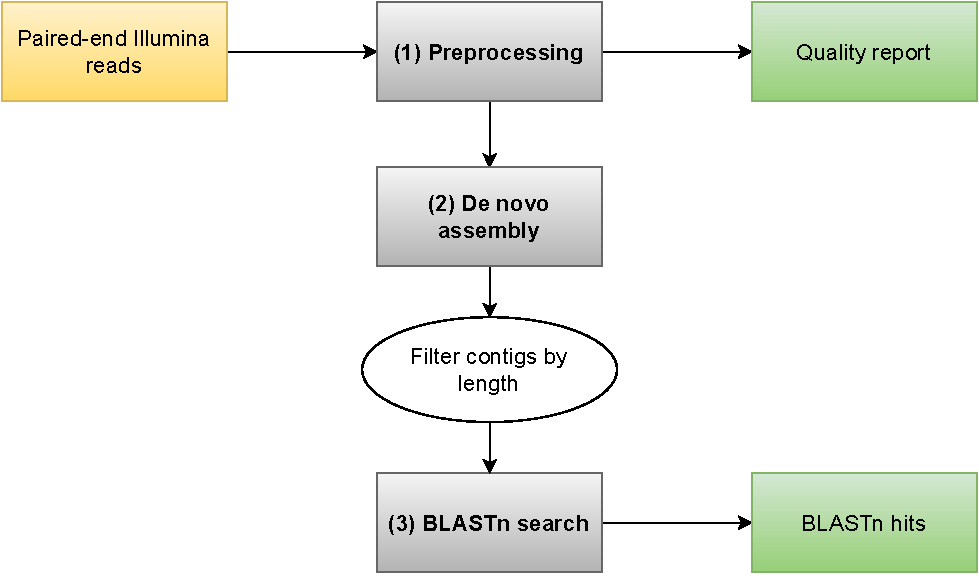
\includegraphics[width=0.9\textwidth]{media/3-fmdv-1-2.pdf}
	\caption{Simplified FMDV workflow (1/2) with \textit{de novo} assembly and BLASTn search.}
	\label{fig:3-fmdv-wf-1}
\end{figure}

\begin{figure}[ht!]
	\centering
	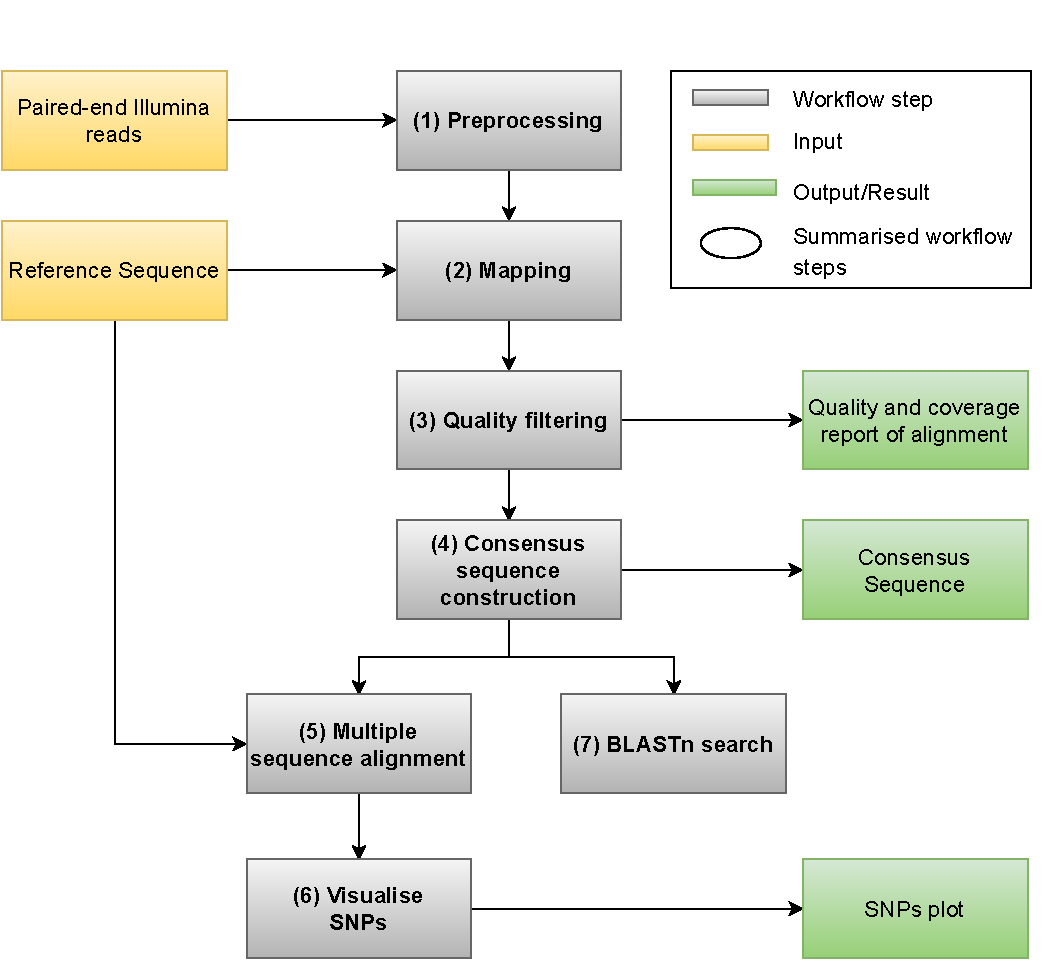
\includegraphics[width=1\textwidth]{media/3-fmdv-2-2.pdf}
	\caption{Simplified \ac{FMDV} workflow (2/2) with reference-based mapping and consensus sequence construction.}
	\label{fig:3-fmdv-wf-2}
\end{figure}
The first part of the workflow accounts for the choice of reference sequence and starts with (1) preprocessing of the reads using \texttt{fastp}. Reads shorter than 30 base pairs are discarded, and polyG tails of the Illumina reads are trimmed automatically. Default settings of \texttt{fastp} account for automatic quality filtering to remove sequencing adapters and unqualified reads by additional quality filters. Before assembly, a step to create a datastructure that allows multisample processing by the assembler is inserted to the workflow. Using the \texttt{Apply Rules} tool, a nested collection from the reads is generated, while each sample is a list containing the forward and reverse reads. This step ensures that the samples are treated separately during assembly and invoke one assembly run per sample.\\
In order to find the most similar existing sequence that can be used as a reference for mapping, this workflow first includes a \textit{de novo} assembly with \texttt{rnaviralSPAdes}. It is an assembler tailored for short \ac{RNA} viral data and was initially developed in a specific version for the assembly of \ac{SARS-CoV-2} samples. It improves the existing \texttt{SPAdes} assembler by making use of knowledge about the structure of viral \ac{RNA} genomes~\cite{meleshko2022coronaspades}. The \ac{FMDV} contigs, which may be varying in terms of amount of sequences and length of contig, are then (2) filtered by length to dismiss short contigs that represent only fragments of the viral genome. The cut-off is set to almost half the size of the \ac{FMDV} (minimal length 4.0 kilobases). This allows the subsequent (3) megablast search on the \ac{NCBI} NT database to find similar nucleotide genomes even in the case of coinfection of the sample or recombination within the viral genome. After the \ac{BLAST} search, the user is required to inspect the top hits, and to identify the best matching reference genome based on their own criteria such as coverage and identity. The resulting sequence that is chosen as a reference may prove plausibility of the sample or reveal the presence of other nucleic material if one of the top \ac{BLAST} results matches an unexpected contaminant. To avoid the automatic choice of reference selection by strictly taking the top \ac{BLAST} match as reference for the following mapping, the workflow is split up into two parts. This implies that if a user has a different reference sequence independent of the first \ac{FMDV} workflow, the sequence analysis can start directly with the second \ac{FMDV} workflow by uploading the reference sequence to a new Galaxy history.

The second workflow for \ac{FMDV} genomic analysis is designed for multiple samples of raw reads in a collection that are mapped to the same reference sequence. This is useful in an outbreak scenario where a workflow user has multiple sequenced samples from the same outbreak and seeks to compare these samples with each other, identify similarities, relations and origin of the virus. However, this workflow can be used as a stand-alone pipeline without the first workflow in case the user aims to map the raw reads to a specific, arbitrarily chosen reference. After uploading the reference sequence in FASTA format, identified from the megablast search and retrieved via the \ac{NCBI} upload tool (\texttt{NCBI Accession Download}) or from other sources, the workflow runs a (1) preprocessing with \texttt{fastp} to dismiss reads shorter than 30 bp and to trim polyG tails of the reads. The second step involves (2) mapping of the preprocessed reads to the reference genome using \texttt{BWA-MEM} with default configurations. This step generates a \ac{SAM} file, which is then (3) filtered for quality using \texttt{samtools}. Paired and mapped reads are kept that have a minimum quality of 20. Alignment and quality reports including coverage statistics are generated per sample using \texttt{QualiMap BamQC}. The filtered \ac{SAM} file is then used to generate a consensus sequence for each sample using the (4) \texttt{iVar consensus} tool with a minimum quality score threshold of 20, minimum frequency threshold of 0.7, minimum indel frequency threshold of 0.7 and a minimum depth of 10 to call consensus. This step allows the workflow to generate a high-quality consensus sequence for each sample, which can be used for downstream analyses, such as multiple sequence alignment and phylogenetic analysis. The resulting consensus sequences from all samples are aligned to the reference genome using (5) \texttt{\acs{MAFFT}}, and this alignment is used to (6) identify and visualise \acp{SNP} with \texttt{snipit}. The \ac{FMDV} workflow produces a summary report of the results of each step and allows the investigation in additional research with the output of each step from within the Galaxy history. 
